\chapter{Additional validation of the MCA}

\label{additional_validation}

Additional validation of the MCA was done by Davide Marenduzzo as described below. A coarse-grained 1D kinetic Monte-Carlo algorithm was constructed. It simulates the diffusion of anionic lipids and the peptide on a 1D lattice. Lipids in the model interact with the peptide via the Debye-Hueckel potential which is truncated at three Debye lengths, whereas the mutual interaction of lipids is neglected. One lattice node can be occupied by multiple lipids. To scale the results of the simulations, it is assumed that the number of 10 lipids per node corresponds to the membrane density of 20\%. Under this assumption, the length unit corresponds to $\sim$6 nm. To achieve equivalence with the standard Brownian dynamics method (without including hydrodynamics, see \cite{Sanz2010}, and references therein), only single particle moves are used. A steady state lipid gradient is created in the same way as it is done in the MCA (chapter \ref{non_uniform_membrane}). Fig. \ref{fig:Davide_simulations} shows that the peptide drifts along the lipid gradient with the velocity that is quantitatively similar to that observed in the MCA. Thus, the effect of the peptide drift is not an artifact of a particular configuration of the MCA in 2D, but it is reproducible with and robust to different implementation details.

\begin{figure}[!ht]
%\centering
%\scalebox{1.0}[1.0]
\begin{center}
  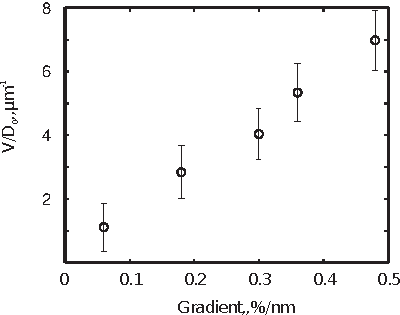
\includegraphics[scale=1.12]{../figures/Davide_simulations.pdf}
\end{center}
 \caption[Peptide drift in the gradient of a monovalent lipid (1D Monte-Carlo simulation model)]{Peptide drift in the gradient of a monovalent lipid in the coarse-grained 1D Monte-Carlo model (taken from \cite{Kiselev2011}). Velocity of the peptide drift is proportional to the lipid gradient.}
\label{fig:Davide_simulations}
\end{figure}